\section{Introduction}
\label{sec:intro}

\epigraph{For five years, Li's formula, known as a Gaussian copula function, looked like
  an unambiguously positive breakthrough, a piece of financial technology that allowed
  hugely complex risks to be modeled with more ease and accuracy than ever before. [...]
  Then the model fell apart.}{\textit{Wired Magazine -- Recipe for Disaster: The Formula
    That Killed Wall Street}}


\subsection{Avant propos}

Il est maintenant indiscutable que l'intersection des statistiques et de l'informatique
joue un rôle fondamental dans la gestion de portefeuille. Ainsi, le \textsl{Wall Street
  Journal}, dans une série consacrée au rôle croissant de l'investissement algorithmique,
déclare que
\begin{displayquote}
  En utilisant des ordinateurs surpuissants pour construire des modèles abscons, ces
  \textit{traders} quantitatifs sont en mesure d'analyser une quantité de données beaucoup
  plus vaste que ce qu'un homme ne pourrait jamais assimiler. Ils siphonnent et classent
  des trillions de gigaoctets de données. Et maintenant, on les entraîne à apprendre de
  leurs succès et de leurs erreurs. [...] Ces \textit{quants} sont devenus si puissants
  qu'ils contrôlent maintenant environ un tiers des échanges sur les marchés boursiers
  américains.\footnote{Traduction de l'auteur. Wall Street Journal, 21 mai
    2017. \textit{Meet the New Kings of Wall Street -- How machines and their masters are
      rewiring the investment world}. Disponible à {\scriptsize
      \url{https://www.wsj.com/articles/the-quants-meet-the-new-kings-of-wall-street-1495389163}}.}
\end{displayquote}
Et pour cause: jamais la puissance de calcul n'a été si impressionnante, ni l'accès à
l'information si peu chère. Construire un modèle d'investissement devient presqu'un jeu
d'enfant, qu'on peut implémenter à peu de frais. Et puis il n'y a qu'à constater que les
plus grands fonds de couverture américains sponsorisent massivement des conférences en
apprentissage machine\footnote{Par exemple : {\scriptsize
    \url{https://nips.cc/Conferences/2016/Sponsors}}}.

Mais alors que chaque fond privé peut y aller de sa propre stratégie, ce ne sont pas là
des modèles universels qui garantissent des revenus sans ne prendre aucun risque. Ou si
c'est le cas, il y a alors une brèche dans l'hypothèse d'absence d'arbitrage qui devra
nécessairement être colmatée par des fonds rivaux. Quoi qu'il en soit, ces
\textit{algorithmes d'investissement} peuvent faire des erreurs et sont forcément exposés
à toute sorte de risques.

La contribution de ce mémoire est de présenter un \textit{algorithme d'investissement}
robuste et souple permettant, non pas de garantir des rendements, mais bien de garantir un
intervalle de rendements possibles, tout en tenant compte des préférences de risque d'un
investisseur. \textit{Grosso modo} donc, ce mémoire propose une décision d'investissement
obtenue par \textit{entraînement} sur des observations du marché qui permet par la suite
de suggérer dans quelle proportion un portefeuille devrait être consacré à un certain
titre risqué.

Cette section fera office d'introduction aux hypothèses qui seront faites et aux questions
qu'on cherchera à résoudre ici. Par la suite, la Section \ref{sec:review} présentera une
revue de littérature consacrée à la gestion de portefeuille dans un contexte statistique
ou mû par les données \textsl{(data driven)}. Puis, la Section \ref{sec:kernel} présentera
en détails l'algorithme permettant de choisir une fonction de décision et les choix qui
doivent être posés afin d'obtenir un modèle satisfaisant. La Section \ref{sec:bound}
enchaînera avec une analyse détaillée des garanties qu'offrent alors une telle fonction de
décision. Ces garanties seront finalement éprouvées dans un cadre expérimental à la
Section \ref{sec:emp}. Enfin, la Section \ref{sec:conclusion} sera l'occasion de conclure
et d'offrir des idées de travaux supplémentaires permettant d'étoffer le modèle.



\subsection{Exposition du problème et hypothèses}

Ce mémoire vise donc à établir clairement et rigoureusement comment un investisseur averse
au risque disposant \textit{d'information complémentaire} au \textit{marché} peut utiliser
cette information pour accroître son \textit{utilité espérée}, qu'on peut traduire par son
\textit{rendement équivalent certain}.

Nous entendrons ici par \textit{marché} n'importe quel type d'actif financier ou
spéculatif dans lequel un investisseur peut investir une partie de sa fortune dans
l'espoir de la voir fructifier au cours d'une période de temps arbitraire. Ainsi, tout au
long de l'exposé théorique qui suivra, il peut être pertinent d'avoir en tête les
rendements quotidiens issus des grands indices boursiers (par exemple les 500 plus grandes
capitalisations américaines). Cependant, le traitement qui sera développé pourrait tout
aussi bien s'appliquer à une action cotée en bourse dont on considère les rendements
mensuels.  Mathématiquement, l'idée de marché peut ainsi être réduite à celle d'un
processus aléatoire $R(t)$ décrivant l'évolution du rendement de l'actif en question.

Relativement à l'idée de marché, nous ferons également l'hypothèse que l'environnement a
une influence sur les réalisations de ces rendements. Il serait par exemple raisonnable de
croire que le cours du pétrole ou le mouvement de certains facteurs économiques puissent
affecter les aléas boursiers d'une compagnie aérienne. De la même façon, l'annonce d'un
scandale industriel pourrait à son tour avoir des répercussions fâcheuses sur la valeur
boursière d'une firme. En outre, il a été montré par Fama et French (voir
\cite{fama1996multifactor}) que le rendement d'une action pouvait s'expliquer comme une
combinaison linéaire de quelques facteurs fondamentaux (la taille de l'entreprise, le
risque de marché et le ratio cours/valeur). On peut alors considérer un vecteur aléatoire
d'information $\vec X(t) = (X_1(t), X_2(t), \dots)$ dont chaque composante représente une
information particulière qu'on appellera \textit{variable de marché}. D'un point de vue
probabiliste, il est donc naturel de considérer la loi jointe entre les rendements $R(t)$
d'une part et $\{\vec X(\tau) \mid \tau < t\}$ l'ensemble des réalisation des évènements antérieurs
à $t$ d'autre part. Le processus joint de ces deux évènements sera désormais défini comme
\textit{la loi de marché}, ou simplement le marché et sera noté $M(t)$.


Mais bien qu'un tel modèle permette de représenter de façon très générale l'évolution d'un
marché, une hypothèse supplémentaire sera formulée : la \textit{stationnarité de la loi de
  marché}.

C'est une hypothèse contraignante qui évacue complètement la notion de temporalité. Les
réalisations antérieures de $M$ n'ont donc plus aucune influence sur ses réalisations
futures. Dans un cadre appliqué, il serait toutefois possible de modifier le vecteur
aléatoire d'information $X$ afin de lui incorporer, par exemple, les réalisations des
$\tau$ périodes de temps précédentes. En choisissant adéquatement $\tau$, un processus
saisonnier pourrait donc être adapté pour respecter les hypothèses de stationnarité.

La stationnarité de $M$ implique également l'absence de probabilité de faillite,
puisqu'elle exclut d'emblée la présence d'un temps d'arrêt. De plus, le marché ne peut pas
non plus être conçu comme un environnement adversariel qui réagirait aux décisions de
l'investisseur. Ceci vient notamment mettre en cause la théorie des marchés efficients
selon laquelle une brèche dans l'absence d'arbitrage serait colmatée par des agents du
marché par effet d'autorégulation. Nous aurons toutefois l'occasion de revenir plus en
détail sur les liens à faire entre cet exposé et l'efficience des marché.

Formellement, nous supposerons que le vecteur d'information $X$ est formé de $p$ variables
aléatoires réelles $(X_1,\ldots,X_p)$ et est supporté par un domaine $\X \subseteq \Re^p$. Les
réalisations de $X$ seront notées $x \sim X$. La variable de rendement aléatoire $R$ sera
supportée par $\R \subseteq \Re$ et une réalisation particulière sera notée $r \sim R$.  La loi de
marché sera ainsi supportée par $\M \coloneq \R \times \X$ et pourra être exprimée par
\begin{equation}
  M = (R,X_1, \ldots, X_p).
\end{equation}

On fera également l'hypothèse qu'un investisseur aura accès à un jeu de données
$\S_n \sim M^n$ formé de $n$ réalisations de $M$. Notons que, du fait de la stationnarité de
$M$, ces observations sont identiquement et indépendamment distribuées. Ce jeu de données,
aussi appelé \textit{ensemble d'entraînement}, sera composé d'une matrice d'information
$\Xi \sim X^n$ telle que $\Xi \in \X^n \subseteq \Re^{p \times n}$ et d'un vecteur de rendement
$r \sim R^n$ tel que $r \in \R^n \subseteq \Re^n$.

\begin{figure}
  \centering
  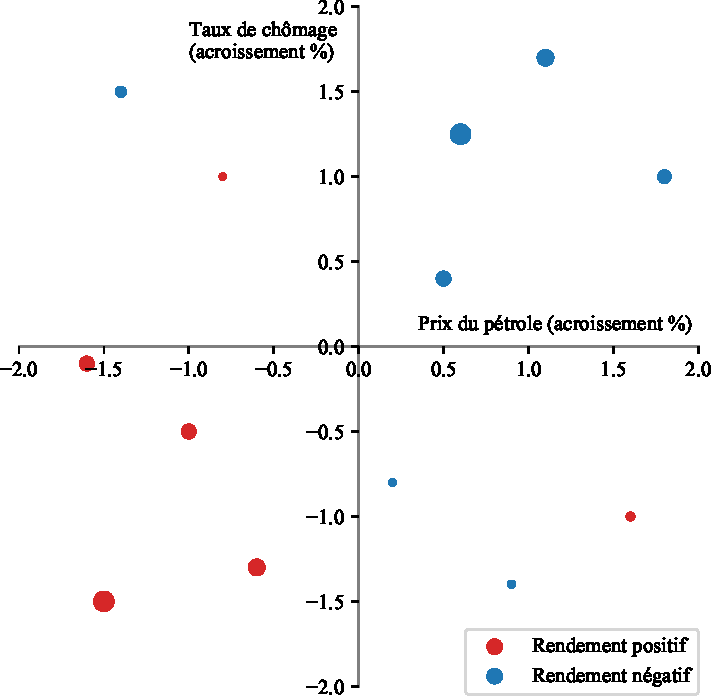
\includegraphics[width=\textwidth]{../experiments/fig/pres/pres1_fr.pdf}
  \caption[Ensemble d'entraînement fictif]{Ensemble d'entraînement fictif sur deux
    variables de marché : le taux de chômage et le prix du pétrole. La taille des points
    est proportionelle à l'intensité des rendements. Cet ensemble est formé des treize
    observations suivantes:\\\\\centerline{ $\Xi = \begin{pmatrix*}[r]
        -1.5 & -1.5 \\
        -1.0  & -0.5 \\
        -0.6 & -1.3 \\
        1.6 & -1.0  \\
        -0.8 &  1.0  \\
        -1.6 & -0.1 \\
        0.5 &  0.4 \\
        1.1 &  1.7 \\
        1.8 &  1.0  \\
        0.6 &  1.25\\
        0.2 & -0.8 \\
        0.9 & -1.4 \\
        -1.4 &  1.5 \\
    \end{pmatrix*},\qquad r = \begin{pmatrix*}[r]
      2.  \\  1.  \\  1.3 \\  0.3 \\  0.2 \\  1.  \\ -1.  \\ -1.3 \\ -0.8 \\
       -2.  \\ -0.2 \\ -0.25\\ -0.5
     \end{pmatrix*}.$} }
  \label{fig_pres1}
\end{figure}

La Figure \ref{fig_pres1} présente une illustration graphique d'un ensemble d'entraînement
fictif qui serait formé de deux variables de marché : le taux de chômage et le prix du
pétrole, et comment celles-ci viendraient influencer les rendements d'une compagnie
aérienne. On y constate que lorsque ces deux variables sont à la hausse, les rendements de
la compagnie chutent, et inversement lorsque les deux variables sont à la baisse. Par
contre, dans la situation où une des deux variable augmente et que l'autre diminue, le
résultat est moins évident.


\subsection{Décision d'investissement et risque de généralisation}

Selon le modèle ici proposé, un investisseur souhaitant investir dans le marché
procéderait de la façon suivante. Dans un premier temps, il prend connaissance des
réalisation des diverses variables de marché $x \sim X$. À partir de cette information, il
décide d'investir une fraction $q(x)$ de sa fortune dans le marché. Puis, le marché
annonce un rendement $r \sim R$. L'investisseur a ainsi réalisé un rendement
$r\,q(x)$. \textit{A priori,} l'investisseur peut donc espérer réaliser un rendement égal
à $\E_MR\cdot q(X)$.

Le problème qui se pose d'emblée est alors de déterminer comment choisir cette
\textit{fonction de décision} $q:\X \to \Re$.

Avant d'aborder ce problème, il faut comprendre que l'investisseur peut disposer d'une
\textit{aversion au risque} qui lui fait préférer des rendements plus modestes mais sûrs à
des rendements en moyenne plus élevés, mais affichant un étalement plus important. Suivant
\cite{von2007theory}, cette préférence sera modélisée à l'aide d'une \textit{fonction
  d'utilité} $u:\R\to\Ut$ dont le rôle est d'attribuer une valeur numérique exprimant la
satisfaction d'un investisseur à l'égard d'un certain rendement $r \in \R$.

En elle même, une utilité de $u(r)$ n'a aucune signification et c'est à l'investisseur de
déterminer une échelle exprimée en \textit{utils}. Par exemple, s'il est averse au risque,
il pourrait accorder à un rendement de -2\% une satisfaction de -10 utils et à un
rendement de 10\% une satisfaction que de 2 utils. De façon absolument équivalente, son
utilité pourrait être calibrée de façon à avoir $u(-2\%) = -1$ et $u(10\%) =
0.2$. L'utilité est donc une notion foncièrement affine et adimensionelle (deux fonctions
d'utilité $u$ et $u'$ sont équivalentes si $u'(r) = ku(r) + b$ pour deux constante $k>0$
et $b$).

Pourvu d'une telle fonction, on supposera alors que l'objectif de l'investisseur sera de
\textit{maximiser son utilité espérée}. Autrement dit, sa fonction de décision $q$ devrait
être choisie de façon à
\begin{equation}
  \label{in:maxeu}
  \maximizeEquation{\EU(q) \coloneq \E_M u(R\cdot q(X)).}
\end{equation}
L'investisseur peut alors espérer réaliser un \textit{rendement équivalent} ou
\textit{équivalent certain} de $u^{-1}(\EU(q))$, où $u^{-1}:\Ut \to \R$ est la fonction
\textit{d'utilité inverse}\footnote{On suppose ici que $u$ est inversible. C'est une
  hypothèse plutôt forte puisqu'elle exclut des formes courantes d'utilité, telle
  l'utilité quadratique de Markowitz.}.

Par contre, étant donné que la forme précise de $M$ n'est pas connue, le problème
\eqref{in:maxeu} ne peut pas être résolu. Il peut néanmoins être approximé en utilisant un
ensemble d'entraînement $\S_n = \{(r_1,x_1),\ldots,(r_n,x_n)\}$ constitué de $n$
observations du marché. L'investisseur cherchera alors à \textit{maximiser son utilité
  espérée en échantillon}:
\begin{equation}
  \maximizeEquation{\hEU(q) \coloneqq n^{-1} \sumi u(r_i\,q(x_i)).}
\end{equation}
La justification théorique d'une telle approximation est la suivante. En notant
$q^\star = \argmax\EU(q)$ la \textit{décision optimale hors échantillon} et
$\qh = \argmax\hEU(q)$ la \textit{décision optimale en échantillon}, l'investisseur
s'assure alors que $\qh \leadsto q^\star$, à mesure que l'investisseur recueille de nouvelles
observations sur le marché (voir \cite{shapiro2009lectures} pour un traitement rigoureux
de l'optimisation stochastique).


\begin{figure}
  \centering
  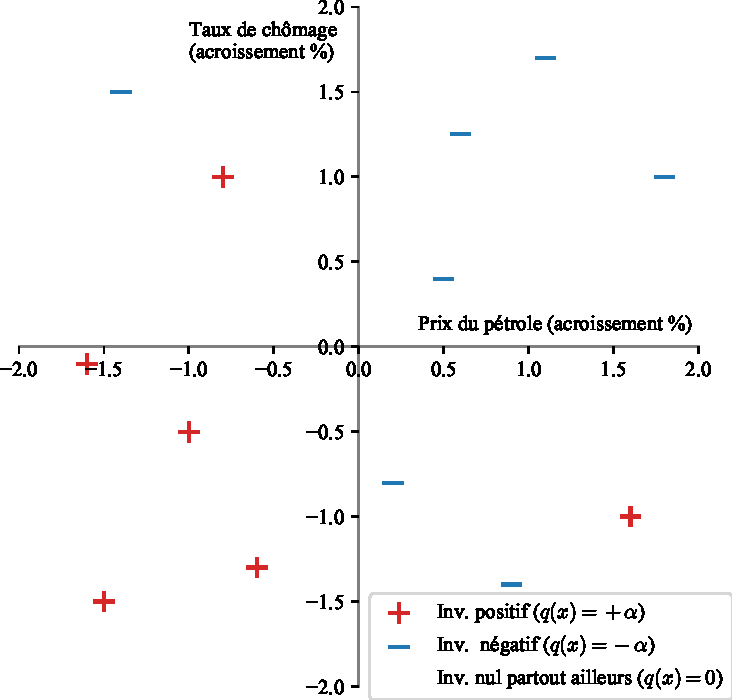
\includegraphics[width=\textwidth]{../experiments/fig/pres/pres2_fr.pdf}
  \caption[Décision ``dictionnaire'']{Fonction de décision ``dictionnaire''. À tout
    rendement positif on associe un investissement positif $q(x)=+\alpha$ et vice versa. On
    obtient ainsi une utilité espérée en échantillon arbitrairement élevée. Par contre une
    telle fonction offre un énorme risque de généralisation puisqu'aucune décision n'est
    prescrite à l'extérieur de l'ensemble $\cup_{i=1}^n\{x_i\}$ des points déjà observés. Si
    $\X$ est dense dans $\Re^2$, alors $q(X)=0$ presque sûrement. }
  \label{fig_pres2}
\end{figure}

L'ennui avec la décision optimale en échantillon, c'est qu'elle souffre d'un important
\textit{risque de généralisation} $\hat\zeta$ défini par
\begin{equation}
  \hat\zeta \coloneq \hEU(\qh) - \EU(\qh).
\end{equation}
Autrement dit, $\qh$ peut mener à une utilité espérée hors échantillon beaucoup plus
faible qu'anticipé par l'utilité moyenne en échantillon.

Considérons par exemple la situation illustrée à la Figure \ref{fig_pres2}. Il suffirait
simplement de définir une fonction $q:\X\to\Re$ préconisant un investissement positif aux
réalisations déjà observées et dont le rendement a été positif et un investissement
négatif dans le cas contraire. Autrement dit, avec $\alpha>0$, cette décision serait construite
de la façon suivante:
\begin{equation}
  q(x) =
  \begin{cases}
     \alpha & \exists\,x_i \in \S_n: [x_i = x \wedge r_i \geq 0]\\
    -\alpha & \exists\,x_i \in \S_n: [x_i = x \wedge r_i < 0]\\
     0 & x \notin \S_n
  \end{cases}.
\end{equation}
Or, si la fonction utilité de l'investisseur n'est pas bornée, une telle fonction de
décision aura nécessairement une utilité moyenne en échantillon arbitrairement élevée à
mesure que $\alpha$ est grand. Par contre, si $\X$ le support de $X$ est dense dans
$\Re^p$, alors l'utilité hors échantillon sera simplement $\EU(q) = u(0)$. Le risque de
généralisation $\hat\zeta$ de $q$ est ainsi arbitrairement grand.

On peut alors faire appel au principe du \textit{rasoir d'Occam} pour éviter que des
fonctions de décision comme celle-ci ne soient favorisées. \textit{Ceteris paribus,} ce
principe suggère en effet qu'une hypothèse trop complexe devrait être découragée au profit
d'une hypothèse plus simple (voir \cite{vapnik1998statistical} pour une discussion
approfondie). Intuitivement, si $\mathscr{C}(q) \in \Re$ mesure la \textit{complexité} d'une
fonction de décision $q$, on pourrait \textit{régulariser} l'objectif pour que
l'investisseur cherche plutôt à
\begin{equation}
  \maximizeEquation{\hEU_\lambda(q) \coloneq \hEU(q) - \lambda\mathscr{C}(q).}
\end{equation}
Différentes valeurs de $\lambda$ favorisent alors des solutions plus ou moins complexes. En
utilisant une technique de \textit{validation croisée} (voir par exemple
\cite{bishop2006pattern}), il y a alors moyen de déterminer le niveau de complexité
permettant de minimiser le risque de généralisation.

\subsection{Espaces de décision et décisions linéaires}

Ce mémoire étudiera les décisions d'investissement obtenues à partir d'un produit scalaire
entre un vecteur de décision $q$ et une observation $x$; le scalaire d'investissement est
alors donné par $q^Tx$. Le problème de maximisation d'utilité espérée s'exprime alors
comme
\begin{equation}
  \label{intro:he}
  \maximizeEquation[q \in \Re^p]{n^{-1}\sumi u(r_i\,q^Tx_i) - \frac{\lambda}{2}\|q\|^2,}
\end{equation}
c'est-à-dire que la \textit{norme} du vecteur de décision $q$ représente la complexité
qu'on lui associe. On comprend alors le rôle que joue alors le facteur de régularisation
$\lambda$. Plus ce facteur est faible et plus la norme de $q$ peut être élevée. Or, comme le
scalaire d'investissement $q^Tx = \|q\|\|x\|\cos\theta$ est directement proportionnel à cette
norme, un facteur de régularisation faible entraînera intuitivement des décisions
d'investissement plus importantes.

Un tel espace de décision est cependant inutilement rigide puisque toute solution ne peut
qu'être linéaire en $\X$, \ie\ $q(0) = 0$. Cette restriction peut être facilement levée en
considérant plutôt des décisions \textit{affines}; il suffit pour ce faire d'ajouter un
terme de ``biais'', \ie\ de déplacement constant au problème d'optimisation:
\begin{equation}
  \maximizeEquation[b \in \Re, q \in \Re^p]{n^{-1}\sumi u(r_i\,(b + q^Tx_i)) - \frac{\lambda}{2}\|q\|^2.}
\end{equation}
On peut aussi tout simplement ajouter une nouvelle variable de marché
$X_{p+1} \sim \delta(1)$ (loi de Dirac constante à $1$), qui permet d'optimiser $q$ directement
sur un espace à $p+1$ dimension.

Finalement, on remarquera que si la fonction $u$ est concave, la présence du terme de
régularisation quadratique fait en sorte que la solution est unique. De plus, le problème
est alors convexe et peut ainsi être résolu numériquement par un solveur standard (par
exemple \cite{cvx,gb08}).

\begin{figure}[p]
  \centering
  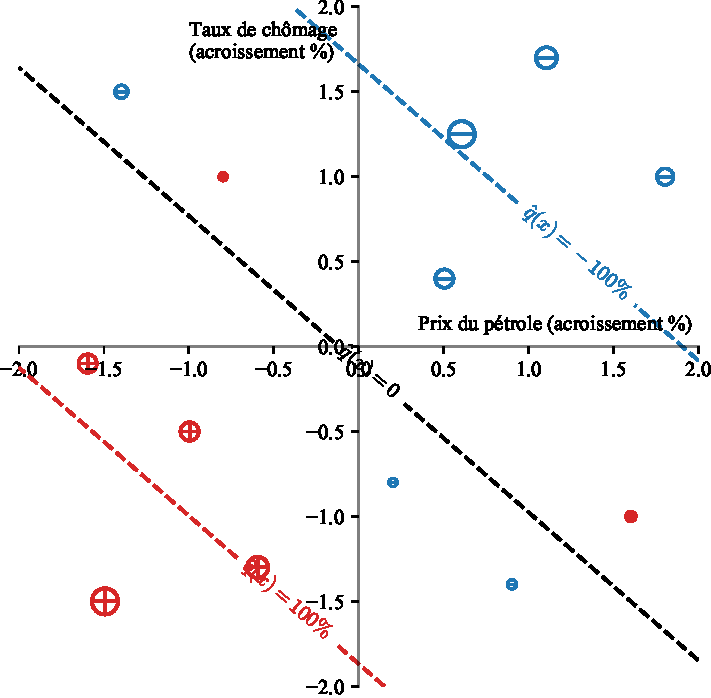
\includegraphics[width=\textwidth]{../experiments/fig/pres/pres3_fr.pdf}
  \caption[Décision linéaire]{Trois courbes d'investissement (-100\%, 0\%, +100\%) de la
    solution linéaire optimale $\qh$ obtenue avec une fonction d'utilité
    $u(r) = -e^{-r}+1$ et un facteur de régularisation $\lambda = 0.3$. La géométrie rigide
    imposée par la forme linéaire de $\qh$ attribue à certaines observations dont le
    rendement est négatif un investissement positif.}
  \label{fig_pres3}
\end{figure}

À des fins d'illustration, la Figure \ref{fig_pres3} présente trois courbes
d'investissement (-100\%, 0\%, +100\%) de la solution optimale $\qh$ obtenues à partir de
l'ensemble d'entraînement de la Figure \ref{fig_pres1}. La géométrie linéaire de $\qh$
entraîne que certaines observations dont le rendement est négatif se voient attribuer un
investissement positif. On verra à la Section \ref{sec:kernel} comment régler ce problème.



\subsection{Objectifs et contributions}

Ce mémoire cherche donc à dégager les principales caractéristiques de cet algorithme
d'apprentissage appliqué à la gestion de portefeuille. Les contributions apportées sont
nombreuses.

D'abord, et c'est son but, cette méthode est parfaitement adaptée pour tenir compte des
informations de marché dont la valeur ajoutée est \textit{a priori} inconnue. Une analyse
de covariance entre ces variables d'information et les réalisations du rendement
permettrait certainement d'en avoir une certaine idée, mais une telle analyse ne tiendrait
pas compte de l'utilité de l'investisseur et ne serait pas régularisée. De plus une simple
analyse en covariance présuppose une dépendance \textit{linéaire} entre les rendements et
les variables de marché. La méthode par noyaux proposée à la Section \ref{sec:kernel}
offre au contraire une richesse supplémentaire au modèle permettant d'exprimer des
situations non linéaires.

Mais c'est aussi le faible nombre d'hypothèses sur la forme de loi de marché (voir Section
\ref{sec:bound}) qui permet à ce modèle de s'éloigner radicalement de l'approche
couramment employée en finance. Par exemple, dans le domaine de la tarification
d'instruments financiers, les rendements sont souvent modélisés selon une distribution
particulière: on peut penser par exemple à l'exemple classique du modèle Black Scholes où
le rendement est distribué selon une simple loi normale (voir
\cite{shreve2004stochastic}), mais également à des modèles plus sophistiqués qui incluent
des processus à saut (voir par exemple \cite{madan1998variance}).

De plus, ce modèle est d'une grande flexibilité puisqu'il accepte toute forme d'utilité
monotone concave et fournit à l'investisseur des garanties probabilistes exprimées en
rendement équivalent sur les erreurs de généralisation et de sous optimalité encourues. En
fait, non seulement ces erreurs sont connues, mais leurs ordres asymptotiques de
convergence le sont eux aussi. Ainsi, un investisseur est en mesure de prédire de combien
peut décroître ou augmenter l'erreur maximale hors échantillon lorsque de nouveaux
échantillons ou de nouvelles variables de marché sont ajoutés pour la prise de décision.

Notons par ailleurs que ce mémoire a aussi le mérite de s'inscrire dans la recherche en
apprentissage statistique en explorant de nouvelles formes de fonction de perte. Deux
classes de problèmes sont traditionnellement considérées : la régression et la
classification. Notre problème emprunte des éléments propres à ces deux classes de
problèmes. D'abord avec la régression puisqu'on cherche dans les deux cas à obtenir une
quantité scalaire. Notre problème en diffère toutefois puisque, contrairement à la
régression où on cherche à \textit{minimiser} la distance entre un estimateur et les
données du problème, l'algorithme d'investissement proposé ici cherche plutôt à
\textit{amplifier} (positivement ou négativement selon le cas) les valeurs (les
rendements) du problème.

On se rapproche également du problème de classification puisque son objectif (non
régularisé) est de la forme
\begin{equation}
  \minimizeEquation[q]{n^{-1}\sumi\ell(y_i\,q^Tx_i)}
\end{equation}
où $y_i\in\{-1,+1\}$ est la cible du problème et $\ell:\Re\to\Re$ mesure l'adéquation entre
$y_i$ et $q^Tx_i$. Typiquement $\ell(z)$ est nul lorsque $z\ge0$, \ie\ lorsque $y_i$ et
$q^Tx_i$ sont du même signe, et est positif (constant ou croissant) dans la région où
$z<0$, \ie\ lorsque $y_i$ et $q^Tx_i$ sont de signes opposés. En fait, la théorie des
machines à vecteurs de support est un cas particulier de notre problème d'optimisation
d'utilité lorsqu'on ne considère que le signe des rendements et qu'on emploie une fonction
d'utilité $u$ nulle sur l'intervalle $[1,\infty]$. Voir \cite{mohri2012foundations} pour une
introduction générale aux problèmes de régression et de classification.

Finalement, ce travail apporte également une modeste contribution au domaine des
statistiques multivariées puisqu'une façon de concevoir le problème de maximisation
d'utilité est comme celui des périls inhérents à l'estimation d'un \textit{vecteur} de
covariance non centrée entre une variable aléatoire scalaire et un vecteur aléatoire. En
effet, dans le cas limite où l'utilité est neutre au risque, \ie\ $u(x) = x$, le problème
de maximisation d'utilité revient à
\begin{equation}
  \maximizeEquation[q]{\E(R\,q^TX) - \tfrac{\lambda}{2}\|q\|^2,}
\end{equation}
dont la solution est donnée par $q =  \lambda^{-1}\E(RX)$, \ie\ la covariance non centrée
entre $R$ et $X$. Ainsi, tous les résultats dérivés dans ce travail s'appliquent aussi à
ce problème d'estimation statistique.



%%% Local Variables:
%%% mode: latex
%%% TeX-master: "memoire"
%%% End:
